\begin{figure}
	\centering
	\begin{subfigure}{0.4\textwidth}
		\centering
		
\includegraphics[width=\linewidth]{figures/hull_a.png}
		\caption{}
		\label{fig:convex_hull_a}
	\end{subfigure}\hspace{12pt}
	\begin{subfigure}{0.4\textwidth}
		\centering
		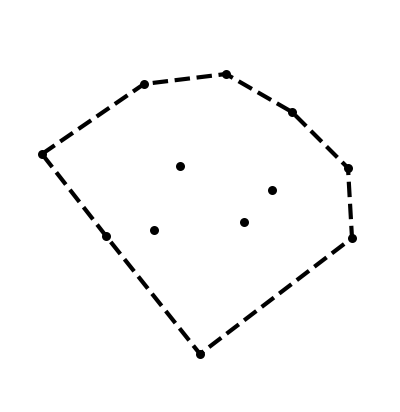
\includegraphics[width=\linewidth]{figures/hull_b.png}
		\caption{}
		\label{fig:convex_hull-b}
	\end{subfigure}
	\caption{A set of points next to their convex hull}
	\label{fig:convex_hull}
\end{figure}
